\documentclass[preprint,12pt,a4paper]{elsarticle}

\usepackage{lineno,hyperref}
\usepackage{float}
\usepackage{subfig}
\usepackage{color}

\usepackage{algcompatible}
\usepackage{algorithm}

\usepackage{cancel}

\usepackage{amsmath,amsthm,amssymb}

\modulolinenumbers[5]

\journal{Computers and Geotechnics}

%%%%%%%%%%%%%%%%%%%%%%%
%% Elsevier bibliography styles
%%%%%%%%%%%%%%%%%%%%%%%
%% To change the style, put a % in front of the second line of the current style and
%% remove the % from the second line of the style you would like to use.
%%%%%%%%%%%%%%%%%%%%%%%

%% Numbered
%\bibliographystyle{model1-num-names}

%% Numbered without titles
%\bibliographystyle{model1a-num-names}

%% Harvard
%\bibliographystyle{model2-names.bst}\biboptions{authoryear}

%% Vancouver numbered
%\usepackage{numcompress}\bibliographystyle{model3-num-names}

%% Vancouver name/year
%\usepackage{numcompress}\bibliographystyle{model4-names}\biboptions{authoryear}

%% APA style
%\bibliographystyle{model5-names}\biboptions{authoryear}

%% AMA style
%\usepackage{numcompress}\bibliographystyle{model6-num-names}

%% `Elsevier LaTeX' style
\bibliographystyle{elsarticle-num}
%%%%%%%%%%%%%%%%%%%%%%%

\begin{document}

\begin{frontmatter}

\title{Meshfree modeling the cyclic behavior of sands with large strain Generalized Plasticity}

%% Group authors per affiliation:
\author{
Pedro Navas$^a$\footnote{Corresponding author: pedro.navas@upm.es},
Diego Manzanal$^a$,
Miguel Mart\'in-Stickle$^{a}$,
and  Manuel Pastor$^a$
 }
 \address{
 $^a$ ETSI Caminos, Canales y Puertos, Universidad Polit\'ectnica de Madrid.\\ c. Prof. Aranguren 3, 28040 Madrid, Spain
}

\begin{abstract}
Several tools are appreciated when the behavior of permeable sands are to be modeled. First of all, since the movement of the water through the solid skeleton is not negligible, the hypotheses made in the $u-p_w$ formulation are not considered, since the acceleration of the fluid take an important place in the studied problem. Thus, the complete formulation plays a significant role in a dynamic problem, taking into account that the employment of an appropriate time integration scheme is essential. On the other hand, when considerable movements of the soil are represented, the combination of large deformation schemes within a meshfree framework is known to provide excellent results. In this way, the implementation of the Generalized Plasticity, suitable for modeling sands under dynamic loads, is presented in this work in a finite deformation framework for the first time.
\end{abstract}

\begin{keyword}
Generalized Plasticity \sep $u-w$ formulation \sep Optimal Transportation Meshfree \sep Soil Dynamics \sep Cyclic
\end{keyword}

\end{frontmatter}

\linenumbers

\section{Introduction}
\label{sec:1}

The Generalized Plasticity model~\cite{PastorZC:90} has been employed successfully in the modeling of sands along the years. Moreover, when cyclic loads appear, this constitutive model is capable to provide useful tools in order to capture the tension-compression states. Several contributions were made in order to improve the original model in different ways: from the implicit integration of the plastic state~\cite{Mira2009} to the inclusion of the softening-hardening of the sands with the employment of the state parameter in saturated~\cite{Manzanal2011} and unsaturated~\cite{Manzanal2011a} ....

MAS SOBRE PZ

MAS SOBRE SANDS-CYCLIC-DRAINED-UNDRAINED

On the other hand, since sands are to be modeled, the intuition make us think that, as the permeability tends to be high, the relative movement of the water phase with respect to the solid one would not be negligible when a dynamic problem, such as a high frequency loading, takes place. Thus, the employment of the traditional $u-p_w$ formulation of the governing equations, even in the dynamic form, is not sufficient to capture the correct acceleration of the water. Zienkiewicz ~\textit{et al.} ~\cite{zienkiewicz1980} made an assessment of the suitability of the usage of the complete formulation depending on the frequency of the loading and the permeability. The dynamic consolidation problems studied in that research were analyzed by Navas ~\textit{et al.} ~\cite{Navas2016b} in the elastic range and also by L\'opez-Querol~\textit{et al.} ~\cite{LopezQuerol2006} within the Generalized Plasticity model for small strains. Therefore, the extension of such formulation to a large deformation framework, within the $u-w$ formulation, is an unquestionable improvement in the field of the cyclic problems of saturated sands. Moreover, the employment of well known meshfree techniques is well indicated when large deformations are involved.

This paper is organized as follows:  In chapter \ref{sec:2} the methodology is presented, being divided in four subsections where the $u-w$ formulation, the time integration scheme, the spatial discretization and the constitutive model are described; the model is calibrated in chapter \ref{sec:3}, being analyzed the monotonic triaxial behavior under drained and undrained conditions test and the cyclic one in chapter \ref{sec:4} for both conditions also. Finally, conclusions are presented in chapter \ref{sec:5}.

\section{Methodology}\label{sec:2}
\subsection{The $u-w$ formulation}
\label{subsec:21}
The main idea of this formulation is the employment of the displacement of the solid and the relative displacement of the fluid as nodal variables. In the literature~\cite{LewisSchrefler98} $\boldsymbol{u}^{ws}$, the relative motion of the fluid with respect to the solid, is defined as $\boldsymbol{  \left(U-u\right) }$, where $\boldsymbol{u}$ and  $\boldsymbol{U}$ respectively stand for displacement vectors of the solid skeleton and the absolute displacement of the fluid phase. The rearrangement of these two gives us the relative displacement of the fluid phase, $\boldsymbol{w}$, with respect to the solid skeleton through the porosity as follows \cite{LopezQuerol2008},
\begin{equation}\label{eq_uw1}
\boldsymbol{ w }=n \boldsymbol{  \left(U-u\right) }.
\end{equation}
being the porosity, $n$ calculated as
\begin{equation}\label{eq_uw3}
n= \frac{V_h}{V_h+V_s},
\end{equation}
where $V_h$ and $V_s$ are the volumes of the voids and solid grains respectively. 
Note that in the current work,   totally saturated porous medium is assumed, i.e., $V_h$ coincides with the water volume, which results in  $S_w$ equal to 1~\cite{LewisSchrefler98}. Thus, similarly, the mixture density, $\rho$, is derived from the ones of the fluid and solid particles, $\rho_w$ and $\rho_s$, as follows:
\begin{equation}\label{eq_uw2}
\rho=(1-n) \rho_s + n \rho_{w}.
\end{equation}

The mass balance equation of the liquid water phase in a isothermal totally saturated media, being compressible water and soil grains and constant the water density, yields ~\cite{LewisSchrefler98}
\begin{equation}
\frac{\dot{ p}_w}{Q} +  \mbox{div }  \boldsymbol{\dot{u}} + \mbox{div } \boldsymbol{\dot{w}} = 0 \label{eq_uw10}.
\end{equation}

  $Q$ represents the volumetric compressibility of the mixture, taking into account that the solid grains are much less compressible than the porous skeleton, is expressed in terms of the bulk modulus of the solid grains, $K_s$, and the compressive modulus of the fluid phase (water), $K_w$, \cite{Zienkiewicz99} i.e.,
 \begin{equation}\label{eq_uw4}
Q = \left[ \frac{1-n}{K_s} + \frac{n}{K_w} \right]^{-1}.
\end{equation}

%%%%%
Equation \eqref{eq_uw10} can be integrated over time to obtain the pore pressure as
\begin{equation}\label{eq_uw15}
p_w=-Q \left[ \mbox{div} (\boldsymbol{u}) + \mbox{div} (\boldsymbol{w}) \right] +p_{w_0},
\end{equation}
where $p_{w_0}$ is the initial pore pressure.
%%%%%

On the other hand, Lewis and Schrefler~\cite{LewisSchrefler98} also give the linear momentum balance equation for the multiphase system under saturated conditions as the summation of the dynamic equations for the individual constituents relative to the solid.
\begin{equation}\label{eq_uw14}
\mbox{div}\boldsymbol{ \sigma} -\rho\boldsymbol{\ddot{u}} -\rho_w\boldsymbol{\ddot{w}}+\rho\boldsymbol{g}=\boldsymbol{0}.
\end{equation}
%%%%

%With respect to the sign criterion for stresses and strains, tensile ones are assumed positive,  except for the pore pressure, $p_w$, which is negative for tension.

 where, taking into account Terzaghi's effective stress theory ~\cite{Terzaghi1925}, the total Cauchy stress tensor, $\boldsymbol{ \sigma}$ can be written in terms of the effective stress, $ \boldsymbol{ \sigma'}$, and the pore pressure, $p_w$, as follows:
\begin{equation}\label{eq_uw5}
 \boldsymbol{ \sigma'} =\boldsymbol{ \sigma} + \alpha p_{w}\textbf{I},
\end{equation}
where  $\textbf{I}$ is  the second order unit tensor.  

Finally, the third Biot's equation is derived from the general form of Darcy's law for any fluid phase:
\begin{equation}\label{eq_uw12}
-\mbox{grad }p_w -\frac{\mu_w}{k}\boldsymbol{\dot{w}}+ \rho_w \left (\boldsymbol{g}-\boldsymbol{\ddot{u}}-\frac{\boldsymbol{\ddot{w}}}{n} \right)=\boldsymbol{0}.
\end{equation}
where $\dot{\boldsymbol{w}}/n$ represents the relative velocity of the fluid, taking into account that $\dot\Box$ is the material time derivative of $\qed$ with respect to the solid; $\boldsymbol{\ddot{u}}$ denotes the solid phase acceleration, $\ddot{\boldsymbol{w}}/n$ is the relative acceleration of the fluid respect to the solid phase, $\boldsymbol{g}$ represents the external acceleration vector, $\mu_w$ denotes the dynamic viscosity of the water and $\boldsymbol{k}$ is the intrinsic permeability tensor, which becomes a unit tensor multiplied by the scalar $k$, intrinsic permeability, when isotropic permeability is assumed.

Both linear momentum balance equations of the mixture and the fluid were presented by Zienkiewicz \textit{et al.} \cite{Zienkiewicz99} with the convective terms, which can be neglected in the present research as the vorticity is relatively small compared to the rest of the terms.

\subsubsection{The weak form of system equations for the $u-w$ formulation}
\label{subsec:21_a}
The weak form of the system equations for the $u-w$ formulation is obtained applying the principle of virtual displacements to the   linear momentum   equation of both the solid and fluid phases, Eqs.~\eqref{eq_uw12} and~\eqref{eq_uw14}.

Taking $\delta\boldsymbol{u}$ and $\delta \boldsymbol{w}$ as the virtual displacement vector for the solid and fluid phase respectively, the weak form of the linear momentum balance equations, once the definition of the pore pressure, $p_w$, of the equation ~\eqref{eq_uw15} is introduced in both Eqs. ~\eqref{eq_uw14} and ~\eqref{eq_uw12} and Green's Theorem is applied, yields:

\begin{eqnarray} \label{eq_uw19_2}
&&-\int_B \boldsymbol{ \sigma'}:\mbox{grad}(\delta\boldsymbol{u}) \, dv \; -\int_B Q \, \mbox{div}(\boldsymbol{u}) \boldsymbol{I}:\mbox{grad}(\delta\boldsymbol{u}) \, dv  - \int_B Q \, \mbox{div}(\boldsymbol{w}) \boldsymbol{I} : \mbox{grad}(\delta\boldsymbol{u}) \, dv
\nonumber \\
&&+ \int_B \left[-\rho\boldsymbol{\ddot{u}}-\rho_w\boldsymbol{\ddot{w}}+\rho\boldsymbol{g}\right]\cdot\delta\boldsymbol{u} \, dv + \int_{\delta B}\boldsymbol{\overline{t}}\cdot\delta\boldsymbol{u} \, ds=0.
\end{eqnarray}

\begin{eqnarray} \label{eq_uw20_2}
&&-\int_B Q \, \mbox{div} (\boldsymbol{u}) \mbox{div}(\delta \boldsymbol{w}) \, dv  -\int_B Q \, \mbox{div} (\boldsymbol{w}) \mbox{div}(\delta \boldsymbol{w}) \, dv \, -\int_B\frac{\mu_w}{k}\boldsymbol{\dot{w}}\cdot\delta \boldsymbol{w} \, dv
\nonumber\\
&&- \int_B \boldsymbol{\ddot{w}}\frac{\rho_w}{n} \cdot\delta \boldsymbol{w} \, dv \, +\int_B \rho_w(\boldsymbol{g}-\boldsymbol{\ddot{u}}) \cdot\delta \boldsymbol{w} \, dv -\int_{\delta B}\boldsymbol{\overline{t}}_w\cdot\delta\boldsymbol{w} \, ds =0.
\end{eqnarray}\\

where $B$ is the volume of the spatial domain and $\delta B$ the boundary where the traction $\boldsymbol{\overline{t}}$ and $\boldsymbol{\overline{t}}_w$, both traction of the solid and fluid phase, are applied.

\subsection{Implicit time integration scheme: Newton-Raphson algorithm}
\label{subsec:22}
In the $u-w$ formulation each node contains both solid and fluid degrees of freedom, $\boldsymbol{u}$ and $\boldsymbol{w}$, whereas the pore pressure, $p_w$ is not considered as a degree of freedom, being calculated at the material point employing Eq.~\eqref{eq_uw15}, in contrast with the more traditional  $u-p_w$ formulation, where is considered directly as an additional nodal unknown. On the one hand, the imposition of impervious boundary conditions is a bit easier in the $u-w$ meanwhile the initial conditions require an initial calculation of the relative displacement of the water, $w$, when an initial pore pressure is assumed. This calculation is further explained in~\ref{ap:1}.

In the proposed study, an axisymmetric 2D configuration is employed in order to represent the triaxial tests. As a two-dimensional problem, the nodal unknowns can be written as:
 $$
 \boldsymbol{u}^*=
 \left[ u_x \quad  u_y \quad   w_x \quad  w_y \right]^T.
$$
After assembling the elementary matrices, the final system of equations can be simplified as
\begin{equation}\label{eq_uw26}
 \boldsymbol{ R}_{k+1}  +  \boldsymbol{C}  \,   \boldsymbol{\dot{u}}_{k+1} +   \boldsymbol{M}   \, \boldsymbol {\ddot{u}}_{k+1}= \boldsymbol{P }_{k+1},
\end{equation}
where   $\boldsymbol{R}$, $ \boldsymbol{C}$ and $  \boldsymbol{ M}$ respectively denote the internal forces vector and damping and mass matrices, whereas $ \boldsymbol{P}$ is the external forces vector, which contains both gravity acceleration and external nodal forces. ${k+1}$ represents the current step.

In order to solve Eq.~(\ref{eq_uw26}) in an implicit way, a traditional Newmark time integration scheme with $\gamma=$0.6 and $\beta=$0.325. (suitable for dynamic problems~\cite{Kontoe2006})is employed. Inserting this scheme into Eq.~(\ref{eq_uw26}),  the equations for the unknowns can be re-written as:
\begin{eqnarray}\label{eq_uw30}
\boldsymbol {G}_{k+1} &=& \boldsymbol {M}\left[\alpha_1\Delta\boldsymbol {u}_{k+1}-\alpha_2\boldsymbol {\dot{u}}_{k}-\alpha_3\boldsymbol {\ddot{u}}_{k}\right] \nonumber\\
&+& 
\boldsymbol {C}\left[\alpha_4\Delta\boldsymbol {u}_{k+1} + \alpha_5\boldsymbol {\dot{u}}_{k} + \alpha_6\boldsymbol {\ddot{u}}_{k}\right] 
\nonumber\\
&+& \boldsymbol {R}_{k+1}-\boldsymbol {P}_{k}-\Delta\boldsymbol {P}_{k+1}=\boldsymbol {0},
\end{eqnarray}

or  in the compact form:
\begin{eqnarray} \label{eq_uw23}
\boldsymbol{G}(\boldsymbol{\chi},\boldsymbol{\eta})&=&\boldsymbol{0},\\
\mbox{where} \quad \boldsymbol{\chi}&=&\left[ \boldsymbol{\chi^u} ,\boldsymbol{\chi^w}\right]^{T} \quad  \mbox{is the deformation mapping}
\nonumber \\
\mbox{and} \quad 
\boldsymbol{\eta}&=&\left[\delta\boldsymbol{u},\delta\boldsymbol{w}\right]^T \, , \; \Delta\boldsymbol{u^*}=\left[\Delta\boldsymbol{u},\Delta\boldsymbol{w}\right]^T.
\nonumber
\end{eqnarray}
where the $\alpha$-parameters are listed in Table~\ref{tab1} according to Wriggers~\cite{wriggers:08}. These coefficients can be easily extended to any other time integration schemes. 

%%%
\begin{table}
\caption{\label{tab1} The $\alpha$-parameters of the Newmark scheme.} 
\centering
	%\vspace*{0.6cm}
	\begin{tabular}{lll}
	 $\alpha_1=\frac{1}{\beta\Delta t^2}$ & 	 $\alpha_2=\frac{1}{\beta\Delta t}$ & 
	 $\alpha_3=\frac{1}{2\beta}-1$ \\
	 $\alpha_4=\frac{\gamma}{\beta\Delta t}$ &  
	 	 $\alpha_5=1-\frac{\gamma}{\beta}$&
	 $\alpha_6=\left(1-\frac{\gamma}{2\beta}\right)\Delta t$
	\end{tabular}
\end{table}

According to Wriggers~\cite{wriggers:08}, to solve the above non-linear equations, any Newton method  can be applied by using the following statement, after the linearization of $ \boldsymbol{\chi}$: 
\begin{eqnarray} \label{eq_uw24}
\boldsymbol{G}(\boldsymbol{\overline{\chi}},\boldsymbol{\eta})_{k+1}^{i}+D\boldsymbol{G}(\boldsymbol{\overline{\chi}},\boldsymbol{\eta})_{k+1}^{i}\cdot \Delta\boldsymbol{u}^{*i+1}_{k+1} &\cong & \boldsymbol{0},
\end{eqnarray}
where $\boldsymbol{\overline{\chi}}$ is the already linearized deformation mapping. Thus, the iterative procedure, taking into account the matrices that are involved in our problem, yields:
\begin{eqnarray}\label{eq_uw32}
\left[\alpha_1\boldsymbol {M}+\alpha_4\boldsymbol {C}+\boldsymbol {K}^{i}_{k+1}\right]\Delta\boldsymbol{u}^{i+1}_{k+1} &=& -\boldsymbol {G}(\boldsymbol {u}^{i}_{k+1}), \\
\mbox{where}\;\; \boldsymbol {u}^{i+1}_{k+1} &=& \boldsymbol {u}^{i}_{k+1} + \Delta \boldsymbol {u}^{i+1}_{k+1}.  \nonumber 
\end{eqnarray}
where $\boldsymbol {K}$ is the tangential stiffness matrix:
\begin{equation}\label{eq_uw31}
\boldsymbol {K}(\boldsymbol {u}^{i}_{k+1})=\boldsymbol {K}^{i}_{k+1}=\left.\frac{\partial\boldsymbol {R}}{\partial \boldsymbol {u}}\right|_{\boldsymbol{u}^{i}_{k+1}}.
\end{equation}
and $i$ depicts the iteration index. The iteration finishes when  $\boldsymbol {G}^{i}_{k+1}$ is lower than a given tolerance.

After applying the integration in time,  Eq.~(\ref{eq_uw19_2}) and Eq.~(\ref{eq_uw20_2}) are written at time $_{k+1}$ and transformed as follows:
\begin{eqnarray} \label{eq_uw34}
&&-\int_B \boldsymbol{ \sigma'}:\mbox{grad}(\delta\boldsymbol{u}) \, dv \; -\int_B  Q \, \mbox{div}(\boldsymbol{u}) \mbox{div}(\delta\boldsymbol{u}) \, dv  \nonumber \\ 
&& -\int_B  Q \, \mbox{div}(\boldsymbol{w}) \mbox{div}(\delta\boldsymbol{u}) \, dv \;  - \alpha_1 \int_B \left[\rho\boldsymbol{u}+\rho_w \boldsymbol{w}\right]\cdot\delta\boldsymbol{u} \, dv 
\nonumber \\
&&+ \int_B \rho\boldsymbol{g}\cdot\delta\boldsymbol{u} \, dv+ \alpha_8 \int_{\delta B} \boldsymbol{\overline{t}}\cdot\delta\boldsymbol{u} \, ds=\boldsymbol{0}
\end{eqnarray}
\begin{eqnarray} \label{eq_uw35}
&&-\int_B Q \, \mbox{div}(\boldsymbol{u}) \mbox{div}(\delta \boldsymbol{w}) \, dv  -\int_B Q \, \mbox{div}(\boldsymbol{w}) \mbox{div}(\delta \boldsymbol{w}) \, dv 
\nonumber\\
&&- \alpha_4\int_B\frac{\mu_w}{k}\boldsymbol{w} \cdot \delta \boldsymbol{w} \, dv 
-\alpha_1 \int_B \frac{\rho_w}{n}\boldsymbol{w}\cdot \delta \boldsymbol{w} \, dv
\nonumber\\
&&-\alpha_1\int_B \rho_w\boldsymbol{u} \cdot \delta \boldsymbol{w} \, dv+\int_B \rho_w\boldsymbol{g} \cdot \delta \boldsymbol{w} \, dv 
\nonumber\\
&&-\int_{\delta B}\boldsymbol{\overline{t}}_w\cdot\delta\boldsymbol{w} \, ds =\boldsymbol{0}.
\end{eqnarray}
The results of the linearization process for  Eq.~(\ref{eq_uw34}) and Eq.(\ref{eq_uw35}) are given in Eq.~(\ref{eq_r1}) and Eq.~(\ref{eq_r2}) respectively in \ref{ap:2}. More details of the linearization process are given in~\cite{Navas:17c}.

%%%%%%%%%%%%%%%%
\subsection{Spatial discretization}
\label{subsec:23}
The shape function employed is based that of Arroyo and Ortiz~\cite{arroyo2006}, who defined exponential  functions based on the principle of  the local maximum entropy (LME).  For a node $a$, it reads,
\begin{equation} \label{eq_N1}
N_a(\textbf{x})=\frac{\exp\left[ -\beta \; |\bf x-x_a|^2 +  \boldsymbol{\lambda}^*  \cdot  (x-x_a)         \right] } {Z(\textbf{x},\boldsymbol{\lambda}^*(\textbf{x}))},
\end{equation}
where
\begin{equation}\label{eq_N2}
Z({\bf x}, {\boldsymbol{\lambda}}) = \sum_{a=1}^{N_b}{ \exp \left[ -\beta \, |{\bf x-x_a}|^2 + \boldsymbol{\lambda}  \cdot  \bf {(x-x_a)}         \right]}.
\end{equation}
$N_b$ represents the neighborhood size. The parameter $\beta$ defines the shape of the neighborhood and $\boldsymbol{\lambda}^*(\bf x)$ comes from the minimization of the function $g(\boldsymbol{\lambda})=\log Z(\bf x, \boldsymbol{\lambda})$ to guarantee the maximum entropy. The first derivatives of the shape function are then obtained from differentiating the shape function itself to get the Hessian matrix \textbf{J}  in the following expression:
\begin{eqnarray}
\nabla N^*_a &=& -N^*_a \,  (\textbf{J}^*)^{-1} \,  (\bf x-x_a) \label{eq_N3}.
\end{eqnarray}
A modified Nelder-Mead algorithm developed by Navas {\it et al.}~\cite{Navas2018} is used for the minimization process in the current work.
 
\subsection{
Hyperelasto-plastic material model: the Generalized Plasticity 
}
\label{subsec:24}
As it was mentioned, the main contribution of this work in the sense of the constitutive model is the implementation of the Generalized Plasticity flow within a large deformation framework. This scheme employs as the main strain measurement the deformation gradient tensor, calculated in an incremental way thanks to the updated lagrangian approach (CITAS, CITAS). For both phases, the increments are calculated with the gradient of the Local Max-Ent shape functions, Eq.~\eqref{eq_N3}, as follows:

\begin{eqnarray}
\Delta \mathbf{F}_{k+1} &=& I+\sum_{a=1}^{Nb}\Delta u_{k+1}^a \nabla N^a(x_{k}^p), \\
\Delta \mathbf{F}^w_{k+1} &=&I+\sum_{a=1}^{Nb}\Delta w_{k+1}^a \nabla N^a(x_{k}^p)
\end{eqnarray}
where the superscript $p$ represents the material point where is calculated and $Nb$ the neighbor nodes of this material point. The deformation gradient can be calculated as:
\begin{equation}
\mathbf{F}_{k+1} = \Delta \mathbf{F}_{k+1} \mathbf{F}_{k} 
\end{equation}
where $k$ and $k+1$ depict the previous and the current step.

The methodology that is employed in this research reproduces the proposed by Navas~\textit{et al.}~\cite{Navas:17c} for the pore pressure and stress update: following the work of Cuiti\~no and Ortiz \cite{cuitino:92} to relate the left Cauchy-Green strain tensor $\mathbf{B}$ and the small strain tensor $\boldsymbol{\varepsilon}$ during the trial step, where $\mathbf{B}=\mathbf{F}\mathbf{F}^T$. Following, the main relationships between large and small strain configurations that are employed herein are presented.

\begin{eqnarray}
\boldsymbol{\varepsilon}^{e\; trial}_{k+1} &=& \frac{1}{2}\,\log\mathbf{B}^{e\; trial}_{k+1},
\\
\mbox{div }(\boldsymbol{u}) &=& \mbox{tr}(\boldsymbol{\varepsilon}_{k+1})=\mbox{tr} \left (\frac{1}{2}\,\log\mathbf{B}_{k+1} \right), \\
\mbox{div }(\boldsymbol{w}) &=& \mbox{tr} (\boldsymbol{\varepsilon}^w_{k+1})=\mbox{tr} \left(\frac{1}{2}\,\log\mathbf{B}^w_{k+1} \right), \\
p_w&=&-Q \left( \mbox{div } \boldsymbol{u} + \mbox{div } \boldsymbol{w} \right).
\end{eqnarray}

One interesting issue of Constitutive laws in soils is its definition by means of \(p^{\prime}, q\) and \(\theta\) stress components, which
are defined as follows:

\begin{eqnarray}
p^{\prime} &=-\frac{1}{3} I_{1} \label{Eq1}\\ 
q &=\left(3 J_{2}\right)^{1 / 2} \label{Eq2}\\ 
\theta &=\frac{1}{3} \sin ^{-1}\left(\frac{-3 \sqrt{3}}{2} \frac{J_{3}}{J_{2}^{3 / 2}}\right)\label{Eq3}
\end{eqnarray}

where \(I_{1}, J_{2}\) and \(J_{3},\) respectively, denote the first invariant of effective stress tensor and second
and third invariants of deviatoric stress tensor. Negative sign in Equation \eqref{Eq1} stands for positive values of \(p^{\prime}\) in compression. However, the sign of $q$ is closely related to the orientation in the triaxial space, \textit{i.e.}, the Lode's angle $\theta$ of the stress path: if $\sin 3\theta$ is lower than 0, we consider the load in tension and the sign of $q$ negative, meanwhile $q$ is positive on any other situation. Working with $p$ and $q$ is an aspect that allows as to reduce the computational effort since only two variables define the stress state of the material point instead of every component of the stress tensor in the cartesian space as it was the traditional way to operate with Generalized Plasticity~\cite{Mira2009}.\\

In the same manner, strains can be defined in the triaxial space taking into account again that the sign of $\varepsilon_s$ will be defined be a conjugate strain Lode\'s angle. The expressions read as follows:
\begin{eqnarray}
\varepsilon_v &=- tr(\boldsymbol{\varepsilon})\label{Eq4}\\ 
\varepsilon_s &=\sqrt{\frac{2}{3}}\Vert \boldsymbol{\varepsilon}^{dev} \Vert \label{Eq5}\\ 
\theta^{\varepsilon} &=\frac{1}{3} \sin ^{-1}\left(\frac{-3 \sqrt{3}}{2} \frac{J^{\varepsilon}_{3}}{J_{2}^{\varepsilon \,3 / 2}}\right)\label{Eq6}
\end{eqnarray}

In this work, the hyperelastic HAR model~\cite{Houlsby2005} has been employed, with the reduced version ($n=1$). The Free Energy function is represented by the following equation:
\begin{equation}
\psi\left(\varepsilon_{v}^{\mathrm{e}}, \varepsilon_{s}^{\mathrm{e}}\right)=\frac{p_{a}}{K_0} \cdot \exp \left(K_0 \cdot \varepsilon_{v}^{\mathrm{e}}+\frac{3 G_0 K_0\left(\varepsilon_{s}^{\mathrm{e}}\right)^{2}}{2}\right)
\end{equation}

Invariants $p$ and $q$ can be calculated from this function taking into account their own derivatives with respect to the strain invariants $\varepsilon_{v}^{\mathrm{e}}$ and $\varepsilon_{s}^{\mathrm{e}}$:


\begin{equation}\label{PZ1}
\left[ 
\begin{array}{c}
p \\ 
q
\end{array}
\right]=
\left[\begin{array}{cc}
\frac{\partial^{2} \psi}{\partial \varepsilon_{v}^{\mathrm{e}\,2}}
 &  
 \frac{\partial^{2} \psi}{\partial\varepsilon_{v}^\mathrm{e} \partial\varepsilon_{s}^\mathrm{e}} 
 \\
 \frac{\partial^{2} \psi}{\partial\varepsilon_{s}^\mathrm{e} \partial\varepsilon_{v}^\mathrm{e}} 
 & 
\frac{\partial^{2} \psi}{\partial\varepsilon_{s}^\mathrm{e\,2}}
\end{array}
\right]
\left[
\begin{array}{c}
\varepsilon_{v}^{\mathrm{e}}
 \\ 
\varepsilon_{s}^{\mathrm{e}}
\end{array}
\right]
\end{equation}

Once defined the hyperelatic part, the plastic behavior is described only with the normal vectors to the yield and the potential surfaces, given  respectively by $n$ and $n_{g}$. The potential vector take different direction depending on the loading or unloading criteria. In the $p, q, \theta $
stress space, these vectors are:
\begin{eqnarray}
n &=\left(n^{p}, n^{q}, n^{\theta}\right)^{\mathrm{T}} \\ n_{g,L} &=\left(n_{g,L}^{p}, n_{g}^{q}, n_{g}^{\theta}\right)^{\mathrm{T}}
\\ n_{g,U} &=\left(n_{g,U}^{p}, n_{g}^{q}, n_{g}^{\theta}\right)^{\mathrm{T}}
\end{eqnarray}
where the components are described in Table \ref{tab2}.

\begin{table}[H]
\caption{\label{tab2} $n_{g}$ and $n$ components.} 
\centering
	\begin{tabular}{l|l}
        $n^{p} =\frac{d_{f}}{\sqrt{1+d_{f}^{2}}}$ &
        $n_{g,L}^{p} =\frac{d_{g}}{\sqrt{1+d_{g}^{2}}}$
        \\ 
         &
        $n_{g,U}^{p} = -\Vert n_{g,L}^{p} \Vert$ \\
        $n^{q} =\frac{\pm 1}{\sqrt{1+d_{f}^{2}}}$ &
        $n_{g}^{q} = \frac{\pm 1}{\sqrt{1+d_{g}^{2}}}$ \\  
        $n^{\theta} =-\frac{q M_{f} \cos 3 \theta}{2 \sqrt{1+d_{f}^{2}}}$ &
         $n_{g}^{\theta} =-\frac{q M_{g} \cos 3 \theta}{2 \sqrt{1+d_{g}^{2}}}$
	\end{tabular}
\end{table}

The dilatancies are represented by $d_{f}=\left(1+\alpha_{f}\right)\left(M_{f}-\eta\right)$ and $d_{g}=\left(1+\alpha_{g}\right)\left(M_{g}-\eta\right)$, taking into account that $M_{g}$ and $M_{f}$ are the slopes of the critical state lines of the potential and yield surfaces respectively and $\alpha_{g}$ and $\alpha_{f}$ are model parameters. $\eta$ depicts the current relation between $q/p$. As we see in Table~\ref{tab1}, the deviatoric component can take positive or negative sign, which depends on the sign of the invariant $q$, if it is in extension (negative) or compression (positive).

The goal of the plastic driver is the calculation of the plastic part of the strain tensor. In the Generalized Plasticity, it can be calculated as:
\begin{equation}
d \boldsymbol{\varepsilon}^{p}=\frac{1}{H_{L / U}}\left(\mathbf{n}_{g L / U} \otimes \mathbf{n}\right) : d \boldsymbol{\sigma}
\end{equation}

Although this assertion is valid for any space, in our case, $d \boldsymbol{\sigma}$ and $d \boldsymbol{\varepsilon}^{p}$ are defined in the triaxial space. On the other hand, $H_{L / U}$ is called the plastic modulus, which is defined in a different way depending on the loading or unloading conditions. In the first case it es plotted as:
\begin{equation}
H=p\,H_{0}  H_{f}\left(H_{v}+H_{s}\right) H_{\mathrm{DM}}
\end{equation}
where $H_0$ is a material parameter that Schrefler and coworkers~\cite{Santagiuliana2006} related to the traditional slopes of the plastic and elastic curves in the $p-e$ curve:
\begin{equation}
H_{0}=\frac{1+e_{0}}{\lambda-k}=\frac{1}{\lambda^*-k^*}
\end{equation}

The rest of the parameters are defined following:
\begin{equation}
\begin{aligned} H_{\mathrm{f}} &=\left(1-\frac{\eta}{\eta_{\mathrm{f}}}\right)^{4} \\ 
H_{v} &=\left(1-\eta / M_{g}\right) \\ 
H_{s} &=\beta_{0} \beta_{1} \exp \left(-\beta_{0} \xi\right) \\ 
H_{\mathrm{DM}} &=\left(\frac{\zeta_{\mathrm{max}}}{\zeta}\right)^{\gamma_{\mathrm{DM}}} \end{aligned}
\end{equation}
where:
\begin{equation}
\begin{aligned} 
\eta_{\mathrm{f}} &=\left(1+\frac{1}{\alpha_{\mathrm{f}}}\right) M_{\mathrm{f}} \\ 
\zeta &=p^{\prime}\left\{1-\left(\frac{\alpha_{g}}{1+\alpha_{g}}\right) \frac{\eta}{M_{g}}\right\}^{-1 / \alpha_{g}} \end{aligned}
\end{equation}
$\zeta_{\mathrm{max}}$ is the maximum value of $\zeta$ along the computation and $\xi$ is the cumulative deviatoric plastic strain, $\int\left|\mathrm{d} \varepsilon_{s}^{p}\right| $. On the other hand, if the process lies on the unloading, H must follow the following equations, depending on the relation $\left|\frac{M_{g}}{\eta_{u}}\right|$, being $\eta_{u}$ the value of $\eta$ in the turning point (loading to unloading):
\begin{equation}
\begin{array}{c}{H_{U}=H_{U 0}\left(\frac{M_{g}}{\eta_{u}}\right)^{\gamma_{u}} \text { if }\left|\frac{M_{g}}{\eta_{u}}\right|>1} \\ 
{H_{U}=H_{U 0} \quad \text { if }\left|\frac{M_{g}}{\eta_{u}}\right| \leqslant 1}\end{array}
\end{equation}

Once the plastic part is solved, strain and stress tensor, in finite deformation, have to be calculated:
\begin{eqnarray}
    \boldsymbol{\sigma} &=& \frac{1}{J}\boldsymbol{\tau}=\frac{1}{J}\left(p\boldsymbol{I}+ \sqrt{\frac{2}{3}}q{n}^{tr}_{k+1}\right) \\
    \boldsymbol{B}^e &=& \exp (\boldsymbol{\varepsilon}_{k+1}^{e})=\exp\left(\frac{1}{3}\varepsilon_{v}^{\mathrm{e}}\boldsymbol{I} + \sqrt{\frac{3}{2}}\varepsilon_{s}^{\mathrm{e}}{n}^{tr}_{k+1}\right)
\end{eqnarray}

In the above equations, $\boldsymbol{I}$ is the identity matrix and $\boldsymbol{n}^{tr}_{k+1}$ is the normalized unit tensor of the trial deviatoric elastic strain tensor, $\boldsymbol{\varepsilon}^{tr, e}_{k+1}$, i.e.,
\begin{equation}\label{eq_dp9}
\boldsymbol{n}^{tr}_{k+1} =\frac{\boldsymbol{\varepsilon}^{tr,e}_{k+1}}{\|\boldsymbol{\varepsilon}^{tr,e}_{k+1}\|}.
\end{equation}

Finally, since the presented procedure presents an implicit time integration scheme, the consistent tangent modulus is obtained by:
\begin{equation}
\boldsymbol{D}^{\mathrm{ep}}=\boldsymbol{D}^{\mathrm{e}}-\frac{\left(\boldsymbol{D}^{\mathrm{e}} n_{g}\right)\left(n \boldsymbol{D}^{\mathrm{e}}\right)}{H+n^{\mathrm{T}} \boldsymbol{D}^{\mathrm{e}} n_{g}}
\end{equation}
where $n_g$ and $n$ have to be converted to the cartesian space and $\boldsymbol{D}^e$ is the consistent tangent moduli of the elastic part, calculated, also in cartesians, by:
\begin{eqnarray}
\boldsymbol{D}^{\mathrm{e}}=D_{11}^{\mathrm{e}} \boldsymbol{I}\otimes \boldsymbol{I}+\sqrt{\frac{2}{3}} D_{12}^{\mathrm{e}} \boldsymbol{I} \otimes \hat{\boldsymbol{n}}+\sqrt{\frac{2}{3}} D_{21}^{\mathrm{e}} \hat{\boldsymbol{}} \otimes \boldsymbol{I} &\nonumber\\ 
+\frac{2 q}{3 \varepsilon_{s}^{\mathrm{e}}} \mathbf{M}_1 +\frac{2}{3}\left(  D_{22}^{\mathrm{e}} - \frac{q}{ \varepsilon_{s}^{\mathrm{e}}}\right)\hat{\boldsymbol{n}} \otimes \hat{\boldsymbol{n}}&
\end{eqnarray}
being $D^e_{\Box\Box}$ the components of the elastic matrix in the triaxial space, Eq.~\eqref{PZ1}, and $\mathbf{M}_1 $ the matrix that relates the total and the deviatoric strain tensors in Voigt notation ($\mathbf{M}_1 \boldsymbol{\varepsilon}= \boldsymbol{\varepsilon}^{dev}$), which is constructed in the following manner:
\begin{equation}
\mathbf{M}_1 = \boldsymbol{1} - \frac{1}{3	}\left( \boldsymbol{I} \otimes \boldsymbol{I} \right)
\end{equation}
where $\boldsymbol{1}$ is the fourth order identity matrix. 

\section{Model calibration}
\label{sec:3}
The calibration consist of the simulation of several tests, under monotonic loading conditions, of a determined soil, comparing to reference undrained results. For the drained part, the goal is discovering the drainage velocity, being also analyzed the behavior of the soil under drained triaxial conditions. These three results are presented following.

\subsection{Monotonic triaxial test: undrained conditions}
\label{sec:31}
The proposed methodology has to be validated first. A triaxial test with dynamic conditions is proposed since there are several results of this kind of test in literature~\cite{PastorZC:90,Zienkiewicz99}. In Fig.~\ref{fig_Geo} a scheme of this test is presented. Because of the symmetry only one quarter of its geometry can be modeled. Thus, boundaries $\Gamma_1$ and $\Gamma_2$ have to constraint the displacement of the solid and fluid in the perpendicular direction. Boundary $\Gamma_3$ is free to move, although the fluid cannot dissipate in that boundary since there is a membrane to avoid it.

%%%%%%
\begin{figure}
\centering
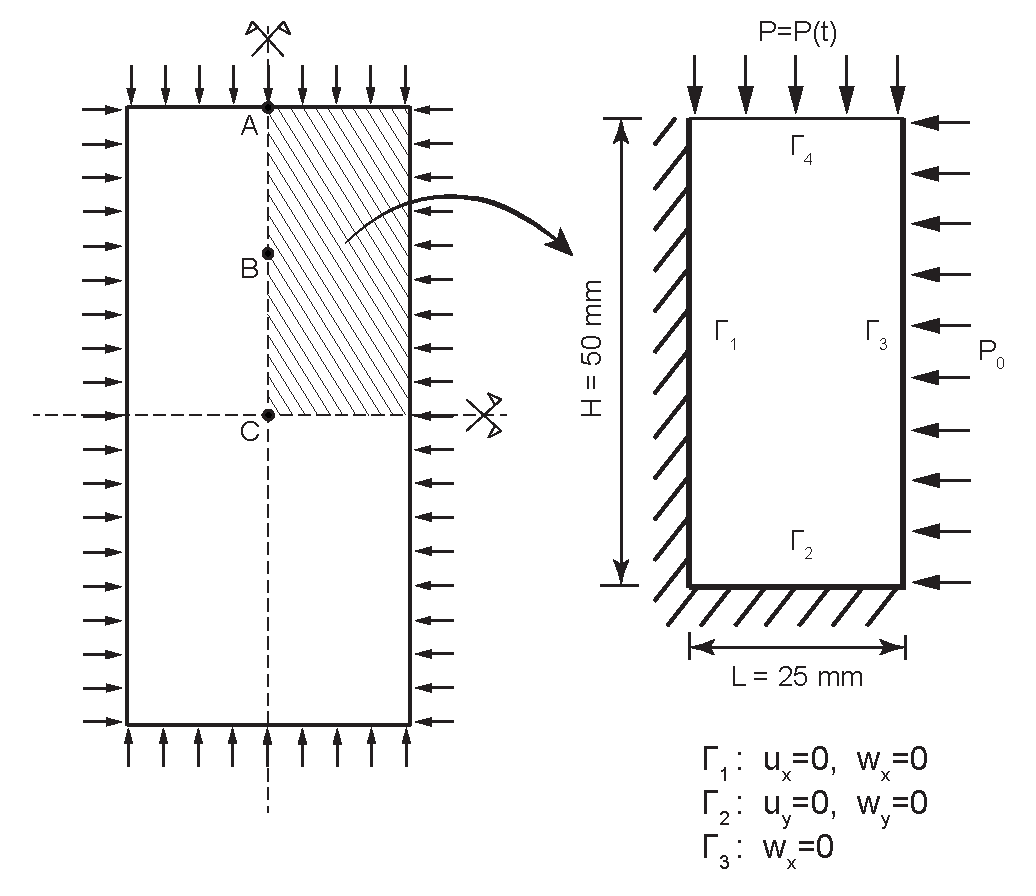
\includegraphics[width=0.85\textwidth]{Figs/Geo.pdf}
\caption{Scheme of the geometry employed in the triaxial test modeling.}
\label{fig_Geo}
\end{figure}
%%%%%%

Boundary $\Gamma_4$ will change depending on the problem to be modeled. About the soil, either the displacement can be imposed or the pressure, if we want to reach a desire value of the $q$. On the other hand, the impermeability of this boundary will be given due to the drained or undrained condition of the reproduced test.

The first test to validate is an undrained monotonic test. The material employed within these tests was a sand studied by Castro (CITA) that, afterwards, was calibrate for the Generalized Plasticity model~\cite{PastorZC:90,Zienkiewicz99}. The parameters that were calibrated are presented in Table~\ref{tab3}. The main 


\begin{table}
\caption{\label{tab3} Material properties employed in the different studied problems.} 
\centering
	\begin{tabular}{l|l}
	& Section 3 \\
	\hline
        $K_{0} \left[ \text{MPa} \right]$  & 35
        \\ 
        $G_{0} \left[ \text{MPa} \right]$ & 52.5
        \\
        \(M_{f}\)  & 0.4
        \\
        \(M_{g}\) & 1.5
        \\
        \(H_{0}\) & 350
        \\
        \(\beta_{0}\) & 4.2
        \\
        \(\beta_{1}\) & 0.2
        \\
        \( \gamma_{u}\)  & -
        \\
        \(H_{u 0}\) & -
        \\
        \( \gamma_{u}\)  & -
        \\
	\end{tabular}
\end{table}

\subsection{Monotonic consolidation test}
\label{sec:32}
Once the behavior of the constitutive model is validated, it is time to verify the performance of the Biot's formulation when the displacement of the water comes into place. Thus, an oedometer, with the geometry proposed in Fig.~\ref{fig_Geo}, is simulated in order to check the consolidation time. A permeability of 1e-6 m/s and a porosity of 0.43 are employed within this simulation. A pressure of 200 kPa is applied to the soil during 0.05 s, point that we consider the consolidation starts. The settlement is obtained from the beginning of the process. The first second of the simulation is presented in Fig.~\ref{fig_conso} for both pore pressure and settlement.
%%%%%%
\begin{figure}
\centering
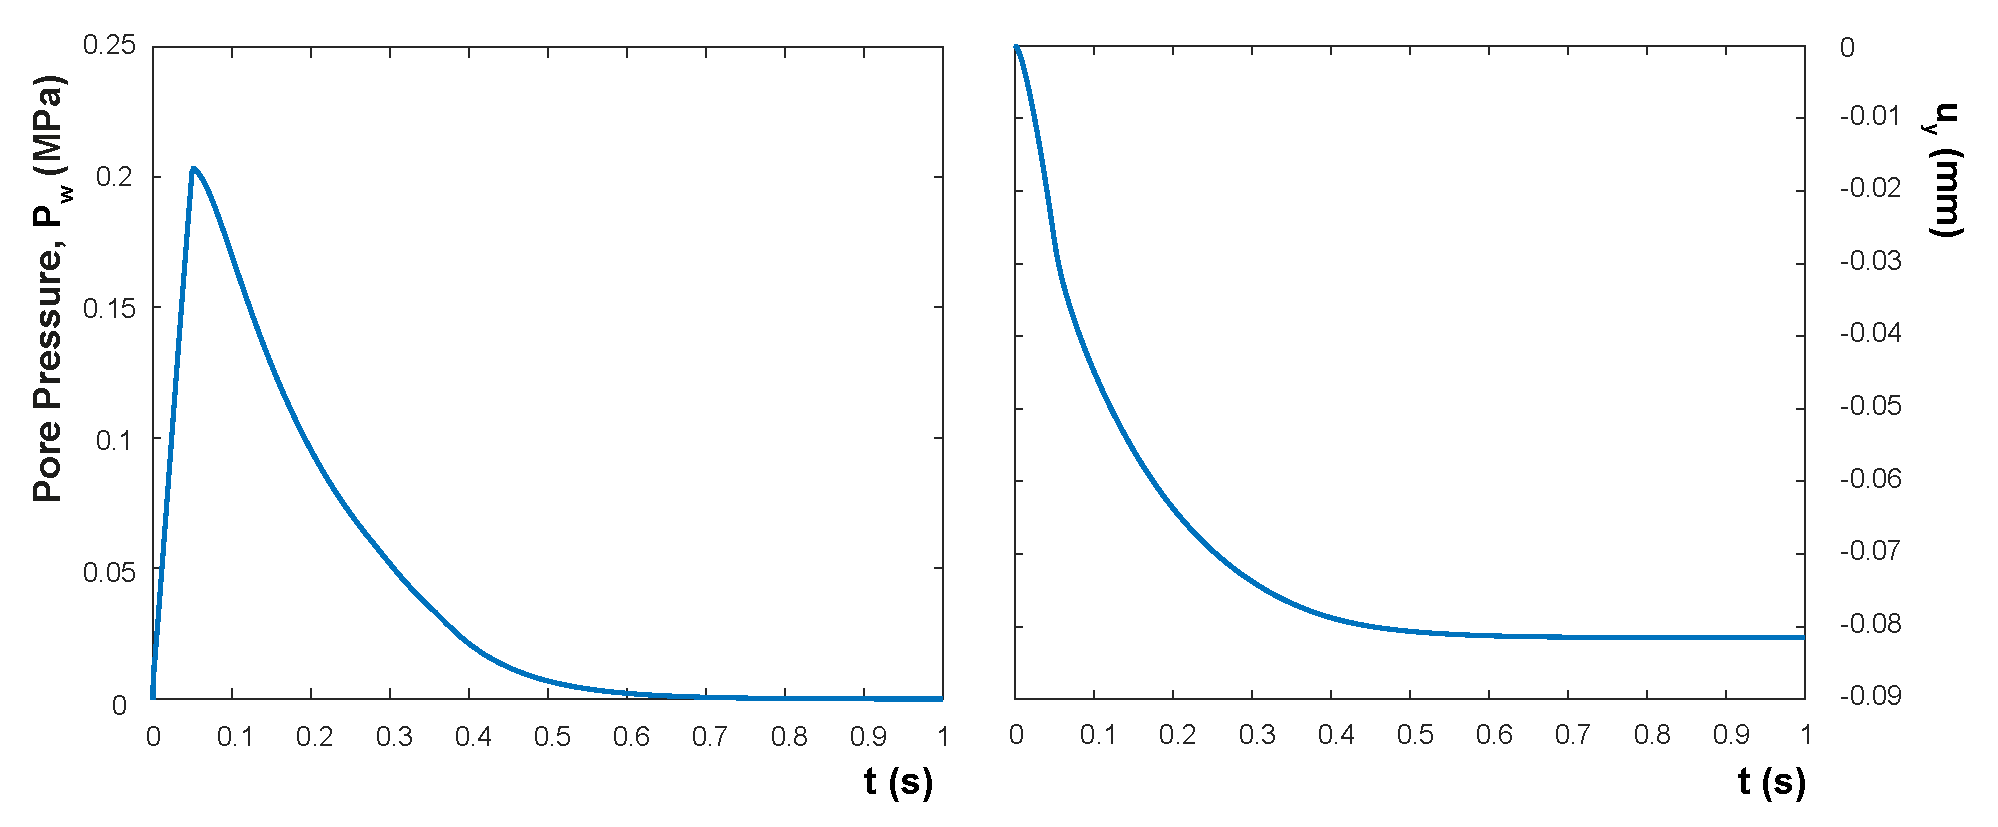
\includegraphics[width=0.95\textwidth]{Figs/conso.pdf}
\caption{Consolidation results: a) Pore pressure, b) Settlement.}
\label{fig_conso}
\end{figure}
%%%%%%

Experimentally, it is demonstrated that the maximum strain rate to obtain drained conditions in a drained triaxial test can be obtained with the following equation:

\begin{equation}
v_{load}=\frac{\varepsilon_f H}{12.7 \, t_{100}}
\end{equation}

\subsection{Monotonic triaxial test: drained conditions}
\label{sec:33}

\section{Cyclic triaxial test}
\label{sec:4}

\subsection{Undrained conditions}
\label{subsec:41}

\subsection{Drained conditions}
\label{subsec:42}

\section{Conclusions}
\label{sec:5}

An interesting methodology to model the dynamic behavior of saturated sands within large deformation is proposed in this paper. Several tools are collected in order to reach the sought behavior of the soil. First of all, the complete $u-w$ large strain formulation developed within an implicit time integration scheme helps us to model the dynamic behavior of saturated sands. Previously, this methodology was proposed with the Optimal Transportation Meshfree with excellent results~\cite{Navas:17c}. Finally, the Generalized Plasticity is well-known to capture properly the behavior of this soil when cyclic loads are involved. However, it was necessary to adapt this model to work in the large deformation framework, which is a big novelty of this work.


The results show excellent performance of the aforementioned tools. Different behaviors were studied in order to assess the suitability of the proposed methodology. The first one, the undrained monotonic one, help us to validate the proposed constitutive model successfully. Following, the limit of the drained-undrained condition is analyzed for the proposed soil and, in chapter 4, the behavior of the model under drained conditions is assessed, verifying that, when the relative motion of the water is not negligible the $u-w$ formulation presents good results. In chapter 5 we could observe the performance of the method under cyclic loads, obtaining the expected behaviors: liquefaction in undrained and densification in drained tests.

The good results obtained in this research encourage us to extend this work in several directions. First of all, since only triaxial tests were carried out, more sophisticated experimental tests as well as real field cases have to be studied with the proposed methodology. On the other hand, several improvements can be made to the constitutive model. The density of the sand in chapter 3 was a relationship between $M_f$ and $M_g$, meanwhile recent developments of the Generalized Plasticity proposed by Manzanal \textit{et al.}~\cite{Manzanal2011,Manzanal2011a} made the densification process in the Generalized Plasticity model more elegant, being able to reproduce the behavior of the soil of the chapter 5.2 easily. Finally, as the methodology is able to capture dynamic behavior, makes sense that the constitutive model were able to capture different behaviors depending on the loading rate with some viscoplastic adjustment, which is something hardly explored within this model. 

\section*{Acknowledgements}
The  financial support to develop this research from the \textit{Ministerio de Ciencia e Innovaci\'on}, under Grant Number, BIA-XXXXX is greatly appreciated. The first author also acknowledges the fellowship Juan de la Cierva FJCI-2017-31544.

\appendix
%\addappheadtotoc
%\appendixpage
%\renewcommand{\theequation}{\Alph{section}.\arabic{equation}}

\clearpage
\numberwithin{equation}{section}
\section{Initial conditions in the $u-w$ formulation}
\label{ap:1}
Some of the triaxial test have, as starting points, initial stress states. In the Generalized Plasticity, it is also necessary to provide this state. Indeed, the stress of this initial point comes from a strain state. The Updated Lagrangian configuration employed within this research needs the previous Deformation Gradient and the current increment in order to situate in the current state. Thus, for the first step we need the tensor $\boldsymbol{F}$ of the initial state. Since no tangential stress takes place we can assume:
\begin{equation}
    \boldsymbol{F}_{ij}=\exp{\boldsymbol{\varepsilon}_{ij}}
\end{equation}
where $\boldsymbol{\varepsilon}_{ij}$ comes from the iterative calculation:
\begin{equation}
    \boldsymbol{\varepsilon}_{ij}=\boldsymbol{D}^{-1}_{ijkl}\:(\boldsymbol{\varepsilon}_{ij})\boldsymbol{\sigma}_{ij}(\boldsymbol{\varepsilon}_{ij})
\end{equation}

The imposition of the initial pore pressure in the $u-w$ formulation is not so straightforward as in the $u-p_w$, where it is a degree of freedom. In the proposed methodology, since it is calculated in the material points with the Eq.~\eqref{eq_uw15}, and the strain state of the soil is defined by the material model, the deformation mapping of the water has to be defined for the initial step, even if there is no initial pore pressure since an equilibrium of Eq.~\eqref{eq_uw15} has to be reached. $\boldsymbol{F}_w$ can be calculated as $\exp{\left[\text{tr}\left(\boldsymbol{\varepsilon}_{w}\right)/3\right]}$, where:
\begin{equation}
  \text{tr}\left(\boldsymbol{\varepsilon}_{w}\right) = \mbox{div} (\boldsymbol{w}) = -\frac{p_{w0}}{Q} - \mbox{div} (\boldsymbol{u})
\end{equation}


\section{Consistent Linearization}
\label{ap:2}
Following, the two main equations of the $u-w$ formulation are presented since these are the equations that are implemented in order to be solved:

\begin{itemize}
\item Linear momentum of for the solid phase
\begin{eqnarray} \label{eq_r1}
&-& \int_B \mbox{grad}(\delta\boldsymbol{u}):\boldsymbol{c}^{ep}:\mbox{grad}(\Delta\boldsymbol{u}) \, dv 
\nonumber \\
&-& \int_B \boldsymbol{ \sigma'}:\mbox{grad}^T(\delta\boldsymbol{u} )\, \mbox{grad}(\Delta\boldsymbol{u}) \, dv 
\nonumber \\
&-& \int_B 
\mbox{grad}(\, \delta\boldsymbol{u}) :\left(Q\left[
%\textcolor{red}{(1-n)}
\mbox{div}(\Delta\boldsymbol{ u})+
%\textcolor{red}{(1-\frac{1}{n})}
\mbox{div}(\Delta\boldsymbol{w}) \right] \boldsymbol{I}\right) dv
\nonumber \\
&-& \int_B 
\mbox{grad}(\, \delta\boldsymbol{u}) : p_w \, \mbox{grad}^T(\Delta\boldsymbol{u}) dv
\nonumber \\
&-& \int_B \mbox{grad}(\, \delta\boldsymbol{u}) : p_w \,\frac{1-n}{n}\mbox{div}(\Delta\boldsymbol{u})\boldsymbol{I} dv
\nonumber \\
&-& \alpha_1\int_B \delta\boldsymbol{u} \cdot \left[\rho \Delta\boldsymbol{u} + \rho_w \Delta\boldsymbol{w} + \rho_w \mbox{div}(\Delta\boldsymbol{u})\left(\boldsymbol{u}+\boldsymbol{w}\right)\right]  dv
\nonumber \\
&+& \int_B \rho_w \delta\boldsymbol{u} \cdot \boldsymbol{g} \, \mbox{div}(\Delta\boldsymbol{u})\, dv
\end{eqnarray}
%%%%%
\item Linear momentum for the fluid phase:
\begin{eqnarray} \label{eq_r2}
&-&\int_B 
\mbox{grad}(\, \delta\boldsymbol{w}) :\left(Q\left[
%\textcolor{red}{(1-n)}
\mbox{div}(\Delta\boldsymbol{ u})+
%\textcolor{red}{(1-\frac{1}{n})}
\mbox{div}(\Delta\boldsymbol{w}) \right] \boldsymbol{I}\right) dv
\nonumber \\
&-& \int_B 
\mbox{grad}(\, \delta\boldsymbol{w}) : p_w \, \mbox{grad}^T(\Delta\boldsymbol{u}) dv
\nonumber \\
&-&\int_B \mbox{grad}(\, \delta\boldsymbol{w}) : p_w \,\frac{1-n}{n}\mbox{div}(\Delta\boldsymbol{u})\boldsymbol{I} dv
\nonumber \\
&-& \alpha_4 \int_B \frac{\mu_w}{k} \delta \boldsymbol{w} \cdot \left[\Delta\boldsymbol{w} + \mbox{div}(\Delta\boldsymbol{u})\left(1-\frac{1-n}{k} \, \frac{\partial k}{\partial n}\right) \boldsymbol{w}\right] \, dv 
\nonumber\\
&-& \alpha_1\int_B\frac{\rho_w}{n} \delta\boldsymbol{w} \cdot \left[\Delta \boldsymbol{w} + \frac{2n-1}{n}\mbox{div}(\Delta\boldsymbol{u})\boldsymbol{w}\right] \, dv
\nonumber\\
&-& \alpha_1 \int_B \rho_w  \delta\boldsymbol{w} \cdot \left[\Delta \boldsymbol{u} +  \mbox{div}(\Delta\boldsymbol{u}) \boldsymbol{u} \right]\, dv
\nonumber\\
&+& \int_B \rho_w \delta\boldsymbol{w} \cdot \boldsymbol{g} \, \mbox{div}(\Delta\boldsymbol{u})\, dv
\end{eqnarray}\\
\end{itemize}



\bibliography{bib2019}

\end{document}